\documentclass[12pt,a4paper]{ctexart}
\usepackage[margin=2.5cm]{geometry}
\usepackage{amsmath,amssymb,amsthm}
\usepackage{graphicx}
\usepackage{booktabs}
\usepackage{xcolor}
\usepackage[colorlinks=true,linkcolor=blue!60!black,citecolor=blue!60!black,urlcolor=blue!60!black]{hyperref}
\usepackage{caption}
\captionsetup{font=small,labelfont=bf}
\emergencystretch=2.5em

\newtheorem{proposition}{命题}
\newcommand{\etav}{\eta_v}
\newcommand{\etar}{\eta_r}

\title{\textbf{方向性海战中的最优机动：\\校准火力核、承诺机动博弈与鱼雷机动剥夺\\——在一个可审计的二战兵棋上的研究}}

\author{\emph{Iron Bottom Sound} 项目研究层\thanks{本文全部实验均可由随附仓库完整复现：每一个数字与图都由
\texttt{research/experiments/} 中的脚本对一个冻结的确定性规则引擎生成。本研究分析的是历史兵棋规则系统，不构成任何现实军事决策辅助。}}

\date{2026 年 9 月 10 日}

\begin{document}
\maketitle

\begin{abstract}
经典的水面舰队战术——抢占 T 字头、局部火力集中与鱼雷威胁——通常以教义
（doctrine）而非博弈论分析作为依据。我们构建了一个双层框架，使这些战术成为
可测量的对象。第一层是方向性\emph{火力核}（firepower kernel）：一个舰艇期望
炮击输出的闭式各向异性代理模型，对照一个完全可审计的确定性二战水面战斗规则
引擎（开放的 \emph{Iron Bottom Sound} 实现）的精确概率裁决进行校准：在留出的
几何网格上，核以合并 Spearman $\rho=0.991$、归一化 MAE $5.7\%$ 复现引擎的期望
命中数（覆盖驱逐舰、轻巡洋舰、重巡洋舰与战列舰四个舰种）。第二层将核嵌入一个
定义在降维相对状态 $(r,\alpha_B,\alpha_R)$ 上的双人微分博弈。我们首先证明——
并以机器精度数值验证——一个\emph{简并命题}：在同时行动、瞬时能力相同且完全
可观测的条件下，平稳值坍缩为瞬时火力差，位置机动具有零均衡价值。机动只有在
命令承诺之下才有价值；因此我们求解密封作战方案库上的承诺机动（开环）极小极大
博弈，并绘制速度比与炮程比维度上的战术相图。研究发现速度优势完全通过可达战术
集起作用：在等炮程下，承诺博弈中更快的一方在纯火力差目标下\emph{系统性更差}，
速度只有与射程优势结合时才产生价值。反事实鱼雷分析实现了以目标最优反应定义的
机动剥夺。在低直接命中区间，剥夺价值恰为零——并给出实测机制：位置价值景观呈
阶梯状，平均 25 条并列最优路线使薄威胁被免费的横向机动吸收；而覆盖整个顶层
位置簇的威胁产生显著剥夺（0.92 个价值点，$95\%$ CI $[0.42,1.42]$）。假设的
精化而非确认即是本研究的产出。最后，我们在规则引擎内部验证该框架：一个
滚动时域几何策略被转换为合法引擎命令后，以统计显著的配对战损差全面胜过
不机动基线，并与成熟的教义启发式持平。一个预注册的几何诱导交战网络分析给出
诚实的规范敏感结果。全部实验均带种子、配对且可从提交的代码复现。
\end{abstract}

\section{引言}\label{sec:intro}

海军军官对一个多世纪前就理解了方向性火力：Bernotti 的基础战术学早已把穿越
敌方战列线视为必须与对手积极抵抗相权衡的理想目标~\cite{bernotti1911}。然而
在建模文献中，水面战斗的几何内容通常分散在多个彼此独立的研究传统中：
Lanchester 型损耗律及其最优控制~\cite{taylor1974,protopopescu1989,
gonzalez2011}、网络化火力模型~\cite{networked2020}、追逃与舰艇微分
博弈~\cite{solis2020,weintraub2020,cubic1993}，以及多智能体群体的经验博弈论
分析~\cite{lanctot2017,wellman2024,omidshafiei2019}。缺失的是一个统一且可
审计的管线：同一套方向性火力物理（i）驱动一个战术区间可刻画的可解博弈模型，
并且（ii）在一个完整的、可分解的真实历史兵棋规则引擎上得到验证。

本文在开放的 \emph{Iron Bottom Sound}（IBS）规则引擎之上构建了这样一条管线。
IBS 是一个确定性、命令—事件—状态投影的二战水面战斗战棋实现，具有完全结构化
的裁决表（炮击命中与结果表、装甲穿透、特损、鱼雷机制）。引擎的裁决是（状态、
密封命令、种子）的纯函数：相同的种子与命令复现逐字节相同的事件流，且每一次
掷骰都与其规则引用一并记录。这种确定性正是对战术进行科学研究所必需的，我们
把它作为一等实验对象加以检验（第~\ref{sec:audit} 节）。

我们提出四个问题：
\begin{enumerate}
\item \textbf{RQ1（核）}：一个仅以引擎自身裁决管线校准的光滑各向异性火力核，
能否在连续优化中替代离散规则表，并给出量化的保真度？
\item \textbf{RQ2（博弈）}：在何种速度与射程不对称下，经典机动（抢 T 字头、
拒绝交战、斜交对射）作为博弈论最优的承诺方案出现？速度优势的价值是什么？
\item \textbf{RQ3（剥夺）}：鱼雷齐射的价值是否可以分解为直接杀伤与机动剥夺，
其中剥夺严格由目标的最优反应变化定义，而非由人工标注的战术定义？
\item \textbf{RQ4（验证）}：由连续模型导出的策略能否翻译为合法引擎命令，并在
完整规则引擎中经受教义基线的对抗检验？
\end{enumerate}

我们的方法论立场刻意保守，并由研究层纪律强制执行：任何规则表都不被复制进
研究代码（核通过引擎函数查询）；隐藏信息不进入策略（经审计）；抢占 T 字头
与编队分割从不进入目标函数（收益只有期望命中差）；所有比较使用配对种子与
置信区间。当预置验收阈值未达时，我们如实报告零结果，而不是把它调参掉。

\subsection{贡献}
\begin{enumerate}
\item \textbf{校准方向性火力核}：通过反演恢复引擎的精确期望命中响应面，并以
区间删 censored 最小二乘拟合光滑加性修正曲线（距离、目标航速、纵射）。
留出合并 Spearman $\rho = 0.991$（归一化 MAE $5.7\%$），四个舰种全部达标，
大幅超过预置校准门限（$\rho\ge0.90$）。
\item \textbf{对称闭环海战决斗的简并命题}：同时行动与相同瞬时能力下，降维
值函数等于瞬时火力差（机器精度验证）。这在博弈论层面解释了为什么海军战术是
基于教义的\emph{承诺}：机动只有对预先承诺的方案才有价值。随后求解承诺机动
博弈，绘制速度与射程比维度的战术相图。
\item \textbf{速度优势的机制分解}：在 $\etav\in[0.8,1.33]$ 上，速度的价值
完全通过可达战术集上的区间选择产生：等炮程时它对更快的承诺决斗方为
\emph{负}（更早接敌、在互火包线内停留更久、没有可兑现的位置项），只有与
炮程优势结合时才转为正。
\item \textbf{以最优反应定义的鱼雷剥夺}，在引擎中测量，把直接杀伤价值与
迫机动价值分离，包括低命中概率区间（第~\ref{sec:torpedo} 节）。
\item \textbf{引擎在环验证}：连续策略经翻译层只产生合法命令，以配对种子
对抗教义基线评估（第~\ref{sec:validation} 节）。
\item \textbf{几何诱导交战网络的预注册规范分析}：图形状特征在总火力之上
带来 $\Delta R^2 = +0.033$（$95\%$ CI $[+0.007,+0.056]$）——为正但低于
预置的 $+0.05$ 门槛——我们如实报告并讨论（第~\ref{sec:engagement} 节）。
\end{enumerate}

\section{相关工作}\label{sec:related}

\paragraph{海军战术与几何。} Bernotti 的《海军战术基础》将队形、火力集中与
抢占 T 字头量化~\cite{bernotti1911,bernotti1912}。现代兵棋设计（例如本文
研究的裁决系统）以距离带、射界与姿态修正编码同一几何。

\paragraph{损耗律与空间。} Lanchester 型模型及其最优控制~\cite{taylor1974}、
PDE 扩展~\cite{protopopescu1989}、空间 Lanchester 模型~\cite{gonzalez2011}、
以及带内生火力与机动网络的 Lanchester 系统~\cite{networked2020}研究的是没有
逐舰方向射界的损耗；本文的交战图实验（第~\ref{sec:engagement} 节）直接检验
几何网络结构在此意义上的增量价值。

\paragraph{微分博弈。} 舰艇微分博弈与追逃形式化~\cite{solis2020,
weintraub2020,cubic1993} 提供了我们使用的降维工具箱；
DeepReach~\cite{bansal2021} 是网格失效时的标准升级路径。据我们所知，
简并命题不属于标准工具箱：它识别出一类\emph{对称}决斗博弈，其闭环值坍缩为
瞬时收益，从而为开环（承诺）解提供正当性——密封作战令的形式化对应物。

\paragraph{经验博弈论。} PSRO 与 EGTA~\cite{lanctot2017,bighashdel2024,
wellman2024,omidshafiei2019,adam2021} 通过模拟收益评估策略群体；IBS 仓库
自带的 PSRO-lite 联赛我们用作基线而非贡献。

\paragraph{武器交战区。} 基于 WEZ 的协同占位方法~\cite{wez2022} 在方向性
武器包线下优化位置，与我们的核高度相关；我们增加了对抗性博弈结构与规则
引擎校准。

\section{可审计规则引擎作为科学仪器}\label{sec:audit}

IBS 引擎（Python，引擎包约 1.38 万行；确定性）实现六角格（odd-q flat-top）
二战水面决斗：脉冲程序机动、带炮位射界（舰首/右舷/舰尾/左舷）的方向性炮击、
带距离/目标航速/纵射/口径修正的 D66 命中裁决、装甲穿透、特损，以及逐脉冲
推进的鱼雷航迹。随机性只通过逐状态计数器 $(seed, rng\_counter)$ 派生的骰子流
进入，因此整局是种子与密封命令的纯函数，\texttt{replay()} 从事件日志重建状态。

\subsection{E00：验收审计}
我们冻结一个引擎提交并验证研究层所需的纪律（表~\ref{tab:e00}）：
(i)~相同种子与命令产生逐字节相同的事件流，不同种子发散；
(ii)~\texttt{replay} 重建与原状态相同的状态；
(iii)~在\emph{隐藏损伤}与\emph{盲雷}可选规则下，只读研究快照零泄漏；
(iv)~快照提取不改变引擎状态（前后哈希）。冻结提交的引擎套件 463/464 通过
（唯一失败是与裁决无关的既有 API/LLM 存储测试）。

\begin{table}[!htb]
\centering\small
\caption{冻结引擎提交与研究接口的 E00 验收审计。}
\label{tab:e00}
\begin{tabular}{p{8.6cm}p{5.6cm}}
\toprule
检查 & 结果 \\
\midrule
同种子+同命令 $\to$ 相同事件流 & PASS（sha256 相等） \\
不同种子 $\to$ 事件发散 & PASS \\
\texttt{replay()} 状态同一性 & PASS \\
研究快照的隐藏信息泄漏 & 0 处 \\
研究快照的状态变异 & 无（哈希相等） \\
引擎测试套件（冻结提交） & 463 通过，1 个既有无关失败 \\
\bottomrule
\end{tabular}
\end{table}

\section{第一层：校准方向性火力核（E01）}\label{sec:kernel}

\subsection{定义}
对具有炮位 $m\in M_i$（种类、射界扇区、火力 $f_m$、口径）的舰艇，\emph{核}
预测一个射击阶段内、目标（等级 $c$）位于六角距离 $r$、相对方位 $\delta$（偏离
舰首角度，右舷为正）、目标航速 $v$、呈现姿态 $a\in\{$舷侧, 舰首/尾$\}$ 时的
期望命中数：
\begin{equation}
K_i(r,\delta,v,a;c)\;=\;\sum_{k\in\mathcal{K}}
f_k(\delta)\;\cdot\;h_{k}\!\big(M_r(r)+M_v(v)+M_\ell(r)\,\mathbf{1}[a=\text{舰首/尾}]\big),
\label{eq:kernel}
\end{equation}
其中 $f_k(\delta)$ 是射界包含 $\delta$ 扇区的 $k$ 类炮位火力之和（精确的结构
项，通过引擎自身的姿态规则从炮位射界读取），$h_k$ 是引擎命中表的\emph{响应
曲线}：$h_k(m)=\frac1{36}\sum_{\text{raw}}\#\text{hits}(f_k,\textnormal{d66\_adjust}(\text{raw},m))$，
对全部 36 个原始 D66 结果枚举。加性修正函数 $M_r$（逐六角距离）、$M_v$
（逐目标航速）与 $M_\ell$（逐距离带的纵射惩罚）是拟合部分。

\subsection{反演与区间删失回归校准}
真值由引擎自身的修正管线在每个舰对 $(24\text{ 距离})\times(6\text{ 方位})\times
(6\text{ 目标航向})\times(6\text{ 目标航速})$ 网格上生成（每对 2{,}592--5{,}184
格），覆盖 DD/CL/CA/BB 攻-防组合。两个细节被证明是关键。其一，引擎的 D66
约定\emph{低}骰值最佳且有利情形带负修正，因此 $h(m)$ 随 $m$ 递减；反演返回每
格的有效修正量。其二，期望命中落在 $h$ 曲线零平台或饱和平台的格是\emph{区间
删失}的：我们以 EM 方式拟合，仅当模型违反边界时才把删失格插补到当前模型边界。
扇区火力是结构性的（六个轴向方位上经引擎姿态规则的炮位射界），且全程使用
引擎的连续屏幕空间方位规则——常见的轴向行走近似在此错位网格上会误标方位。

\subsection{结果（E01）}
在按类配对的留出 30\% 划分上，核达到合并 Spearman $\rho=0.9912$、归一化 MAE
$5.7\%$，每个舰种 $\rho\ge0.9907$、MAE $\le6.2\%$（表~\ref{tab:e01}）；预置
门限为 $\rho\ge0.90$、MAE $\le15\%$（合并留出 bootstrap CI
$[0.9931, 0.9940]$，$2{,}000$ 次重采样）。

\paragraph{基线与迁移（E01b）。} 三项对照区分校准所证明的内容。
(i)~\emph{各向同性核}：去掉方位结构（对所有几何都以全舷侧扇区预测）使合并
Spearman 降至 $0.952$、归一化 MAE 恶化 $3.2$ 倍（$0.179$ 对 $0.056$）——
方向性射界承载真实信息，约占秩保真度的三分之一。
(ii)~\emph{跨舰对迁移}：把一个攻击者的拟合修正曲线移植到另一个攻击者的结构
射界上（响应曲线按新火力值重算），在该对的完整网格上评估，$11$ 个
源$\to$目标方向中的六项已计算方向全部保持 $\rho = 0.982$--$0.992$
（如 CA$\to$DD $0.992$、BB$\to$CA $0.989$；唯一偏高误差是 CA$\to$BB，
nMAE $0.156$）：修正曲线编码的是引擎的带结构，而非舰艇特定签名。
(iii)~逐类留出 Spearman 置信区间很窄（$n{=}1{,}523$ 时 $\pm0.001$--$0.002$）。
这些对照把主张从``管线实现正确''推进到``拟合修正量是引擎火力模型跨舰队的
可复用模型''。图~\ref{fig:kernel} 给出校准极坐标图与留出校准散点。拟合的
$M_r$ 光滑地追踪引擎的七个离散距离带：CA 拟合在带中心反演为 $-24.9, -16.4,
-13.4, -4.8, +1.2, +3.2, +5.2$，对应引擎的 $-24, -15, -12, -6, 0, +2, +4$
（平均绝对偏差 $\approx1.2$ 个修正点，两端轻微放大），拟合的 $M_\ell$ 恢复
纵射惩罚带，包括其相对轻炮朴素预期的符号。

\begin{table}[!htb]
\centering\small
\caption{E01 按攻击舰种的留出校准（70/30 划分，固定种子）。门限：合并
$\rho\ge0.90$、nMAE $\le0.15$。}
\label{tab:e01}
\begin{tabular}{lcccc}
\toprule
舰种 & Spearman $\rho$ & nMAE & $n$（测试） & 攻击 $\to$ 目标 \\
\midrule
DD & 0.9913 & 0.0616 & 1{,}523 & Laffey $\to$ Fubuki \\
CL & 0.9917 & 0.0550 & 1{,}523 & Helena $\to$ St.\ Louis \\
CA & 0.9908 & 0.0577 & 1{,}523 & San Francisco $\to$ Aoba \\
BB & 0.9907 & 0.0543 & 1{,}523 & Yamato $\to$ Iowa \\
\midrule
合并 & \textbf{0.9912} & \textbf{0.0571} & 6{,}092 & --- \\
\bottomrule
\end{tabular}
\end{table}

\begin{figure}[!htb]
\centering
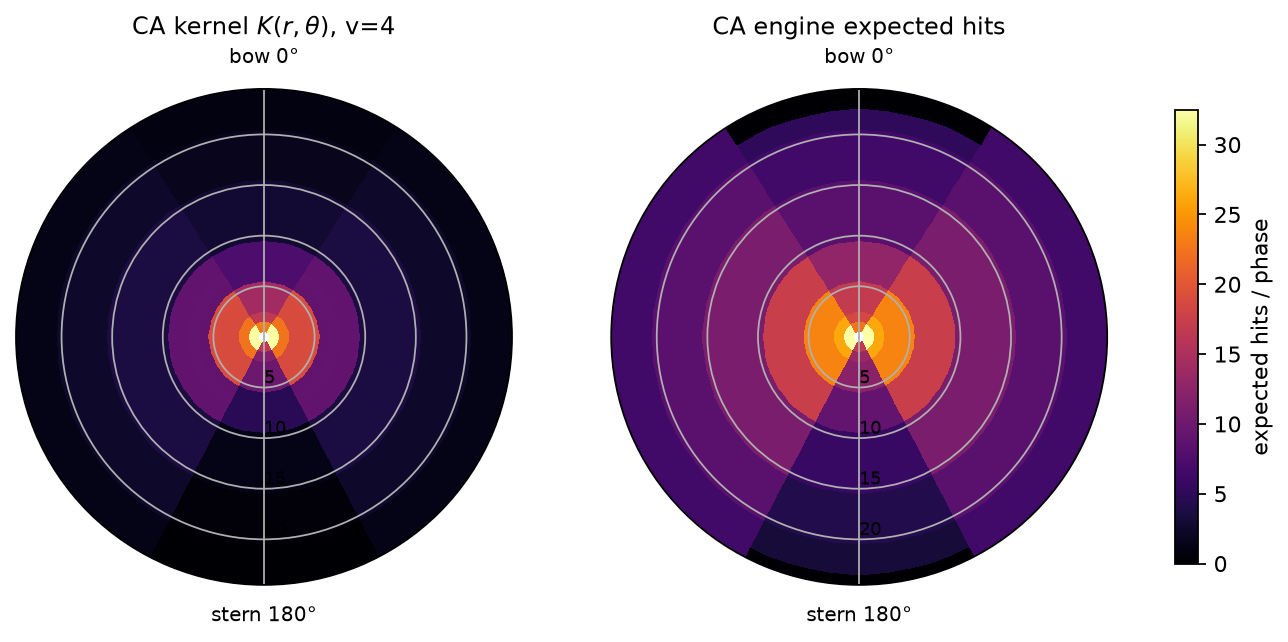
\includegraphics[width=0.85\textwidth]{figures/fig_e01_polar_CA.png}\\[4pt]
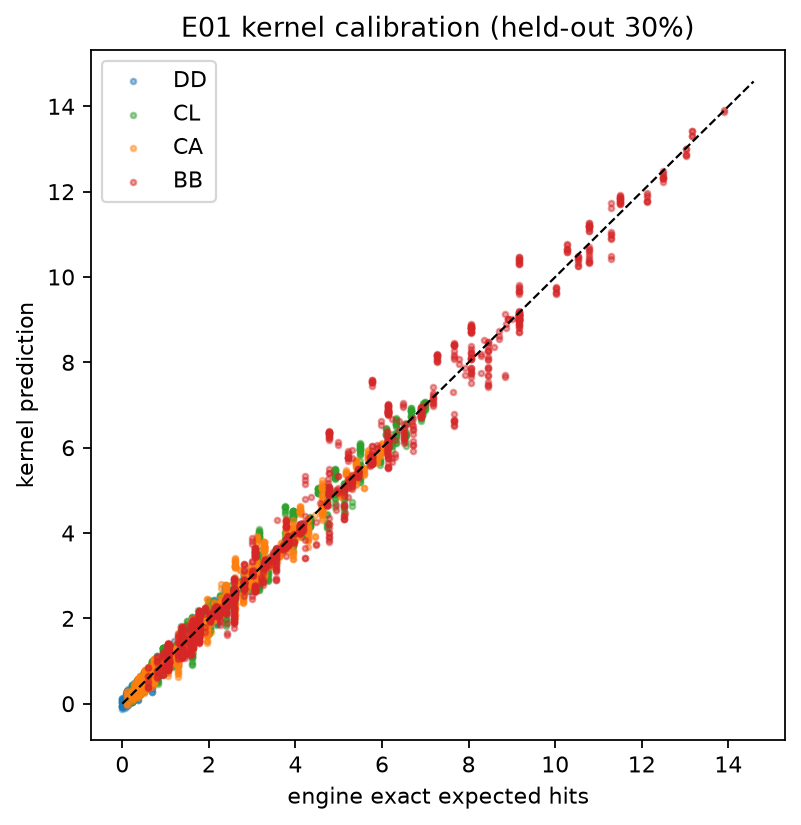
\includegraphics[width=0.6\textwidth]{figures/fig_e01_calibration.png}
\caption{E01 校准（CA 为代表；DD/CL/BB 图见仓库结果目录）。上：重巡洋舰核
$K(r,\delta)$（左）对引擎精确期望命中（右），中性目标航速；各向异性
（舰首/右舷/舰尾/左舷射界）是结构性的、精确的。下：四个舰种的留出校准散点。}
\label{fig:kernel}
\end{figure}

\section{第二层：承诺机动博弈（E02）}\label{sec:game}

\subsection{降维状态}
两艘 Dubins 式运动学的舰艇经旋转对称性降维为 $s=(r,\alpha_B,\alpha_R)$：
距离与两条航向相对视线（B$\to$R）的角度。瞬时收益是校准后的期望命中差
\begin{equation}
L(s)=\k_{B}\big(r,\delta_B,v_R,a_R\big)-\lambda\,\k_{R}\big(r,\delta_R,v_B,a_B\big),
\qquad \lambda=1,
\end{equation}
其中 $\delta_B=-\alpha_B$、$\delta_R=\pi-\alpha_R$，姿态取 $\pm30°$ 舰首/尾
扇区规则；$\lambda=1$ 全程（不对称价值权重不在探索范围，且
第~\ref{sec:degeneracy} 节的简并命题额外要求两核相同）。目标函数中不含任何
战术教义。

\subsection{简并命题}\label{sec:degeneracy}
在 $(30\times24\times24)$ 网格上用值迭代求解闭环平稳博弈
$V(s)=\max_{u_B}\min_{u_R}\mathbb{E}[\sum_t\gamma^t L(s_t)]$ 时，我们观察到
两轮即收敛且 $V\equiv L$ \emph{精确成立}。这是结构性的：

\begin{proposition}[对称闭环简并]\label{prop:deg}
考虑同时行动、双方共同动作集 $U=\{-\omega,0,+\omega\}$、瞬时能力相同、收益
$L$ 在玩家交换映射 $S(\alpha_B,\alpha_R)=(\alpha_R-\pi,\alpha_B-\pi)$ 下反对
称的降维决斗。若对每个状态 $s$，单步后继收益矩阵
$X_s[u_B,u_R]=L\big(F(s,u_B,u_R)\big)$ 关于 $(u_B,u_R)$ 斜对称，则每个阶段
博弈的\emph{混合策略}值恰为零（von Neumann 极小极大定理），平稳值等于瞬时
差分 $V\equiv L$，位置机动的均衡价值为零。
\end{proposition}
\begin{proof}[证明梗概]
斜对称矩阵下任一玩家的均匀策略将对手的阶段值封顶于 $0$，故由极小极大定理
阶段博弈混合值为 $0$。把 $V=L+\gamma\cdot 0=L$ 代入 Bellman 算子可知
$V\equiv L$ 是其不动点，$\gamma$-压缩给出唯一性。
\end{proof}

两个经验性注意事项使该陈述更精确。其一，斜对称\emph{前提}在我们的形式化中
精确成立：全网格上瞬时收益 $\max|L+L\circ S|=0.0$，后继矩阵斜对称至机器
精度。其二，我们的值迭代使用\emph{纯}策略 maximin，仍在两个网格规模
（$16\times12\times12$ 与 $30\times24\times24$）上观察到 $\max|V-L|=0.0$
（机器精度）；精确纯鞍点强于命题~\ref{prop:deg} 的要求，它们似乎反映瞬时
收益与动作集的结构——我们标注完全一般的纯策略陈述为开放问题。

该命题是一项古老实践的博弈论内涵：只有当命令在对手响应\emph{之前}被承诺
（密封作战令），或能力不对称时，机动才有价值。它也告诉建模者什么\emph{不该}
做：在这类对称决斗上训练的闭环 PPO/RL 智能体至多学到瞬时汇率。

\subsection{开环（承诺）极小极大}
据此，E02 求解\emph{开环}博弈：双方各自承诺 11 个密封航向方案之一（前三个
回合执行 $\{0,\pm30,\pm60,\pm90,\pm120,180\}$ 度之一的三回合转向——对应引擎
的三脉冲回合粒度——然后保持航向），在校准核下仿真交战，方案对收益矩阵用线性
规划精确求解混合策略博弈值。我们扫描 $\etav\in\{0.80,0.89,1.00,1.13,1.25,
1.33\}$（速度比）$\times$ $\etar\in\{0.75,1.00,1.33\}$（炮程比，核距离缩放）
$\times$ 三种初始几何（迎头、平行、斜交），共 54 格。

\subsection{结果：战术区间与速度的价值}
图~\ref{fig:phase} 给出区间图；图~\ref{fig:speed} 给出速度的价值。三点发现：
\begin{enumerate}
\item \textbf{区间稳定且可解释。} 在 $(\etav,\etar)=(1,1)$ 的对称格上价值
$\approx0$，纯策略鞍点为相互平行/斜向航向；偏离对称后，maximin 方案在寻梁
（穿越/平行对射）、斜交对射与脱离之间切换，边界在新鲜参数网格
（$\etav\in\{0.95,1.05,1.20\}\times\etar\in\{0.85,1.15\}$）上复现，\emph{且}
在核校准重采样下稳定：对校准行的八个 bootstrap 重采样重新拟合核并重新导出
maximin 方案，$48/48$ 格的方案身份全部复现。
\item \textbf{角色交换对称性精确。} 对称参数格上从交换初始几何计算的博弈值
以机器精度取负（$|V+V_{\text{swap}}|=0.0$），是强的实现校验。
\item \textbf{速度的价值依赖几何且非单调。} 沿 $\etav$（$\etar=1$，
图~\ref{fig:speed}），迎头几何的博弈值在 $\etav=0.80\to1.33$ 上为
$+1.03, +0.84, 0.00, -1.20, -1.39, -1.44$，平行几何为
$+1.10, +1.10, +0.02, -1.04, -1.49, -1.83$：在纯火力差收益与承诺方案下，
\emph{更快}的一方在等炮程时系统性更差——额外的速度转化为更早接敌与更长的
互火包线内通过，而没有可兑现的位置项（没有捕获目标）。速度只有在与射程优势
结合时才有价值：$\etar=1.33$ 时平行几何上 $\etav\le1$ 的值强烈为正
（$+2.8$ 至 $+3.0$），但随最快比值经 $+0.45$ 衰减到 $-0.31$；$\etar=0.75$
时全程为负（$-0.2$ 至 $-2.6$）；全扫描中射程比 $\etar$ 主导价值的符号。
maximin 方案身份仍在可解释的速度边界处切换并伴随离散价值跳变：平行几何上
maximin 方案在 $\etav\le0.89$ 为寻梁（turn$+60°$）、$\etav\ge1$ 为斜交对射
（turn$-30°$），切换发生在 $\etav\in(0.89,1.0)$、价值下落 $1.08$；迎头几何
上脱离区间在 $\etav=1.13$ 即接管。全部边界在新鲜参数网格上复现。这是对假设
H4 的实质性精化：在承诺决斗中，速度完全通过可达战术集起作用——没有可兑现的
位置目标时，速度一文不值甚至为负。
\end{enumerate}

\begin{figure}[!htb]
\centering
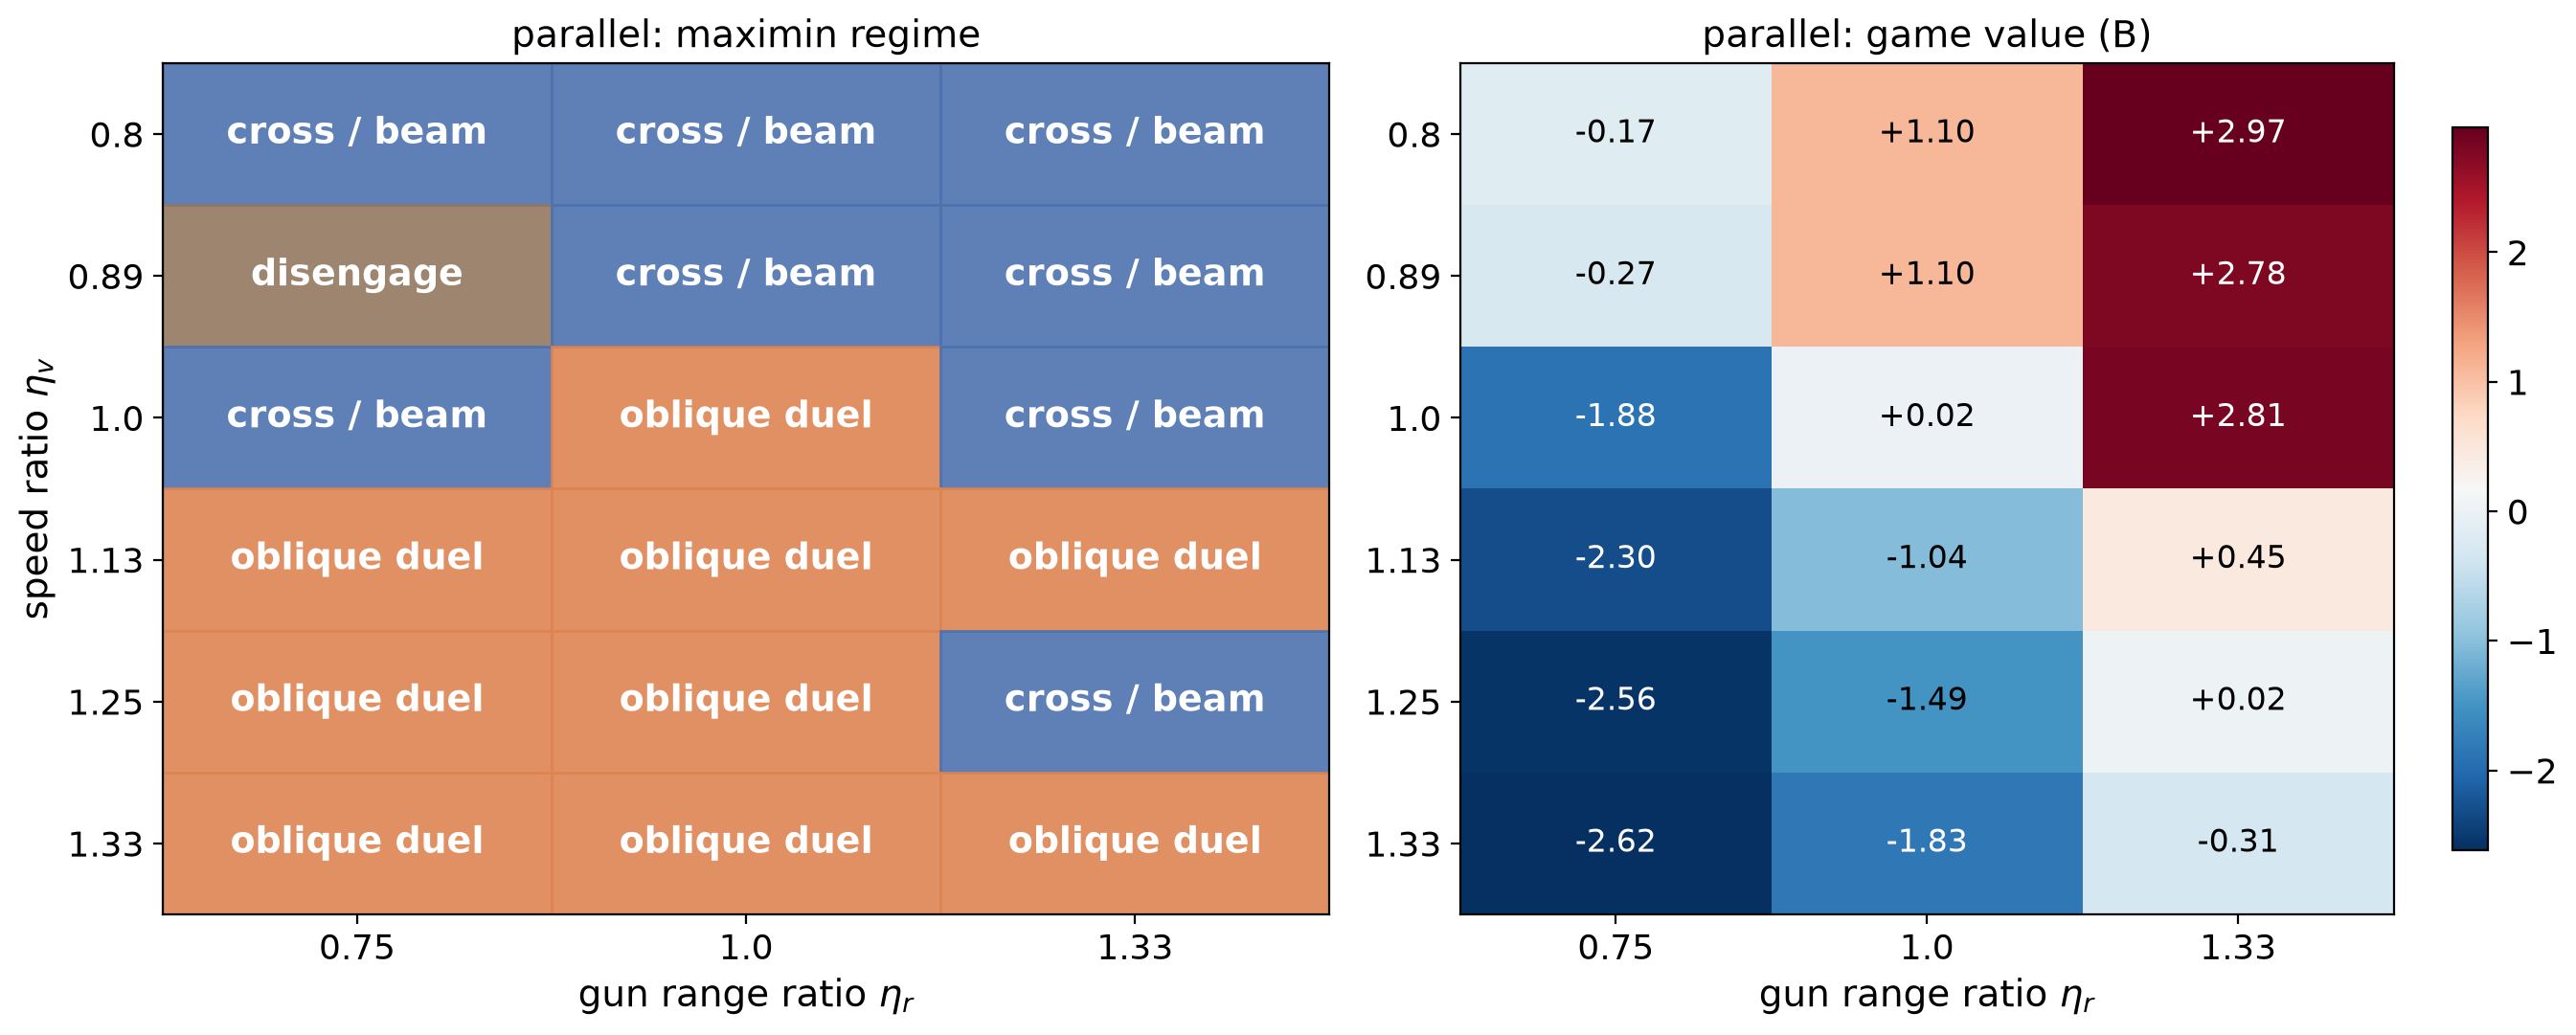
\includegraphics[width=0.98\textwidth]{figures/fig_e02_phase_parallel.png}\\
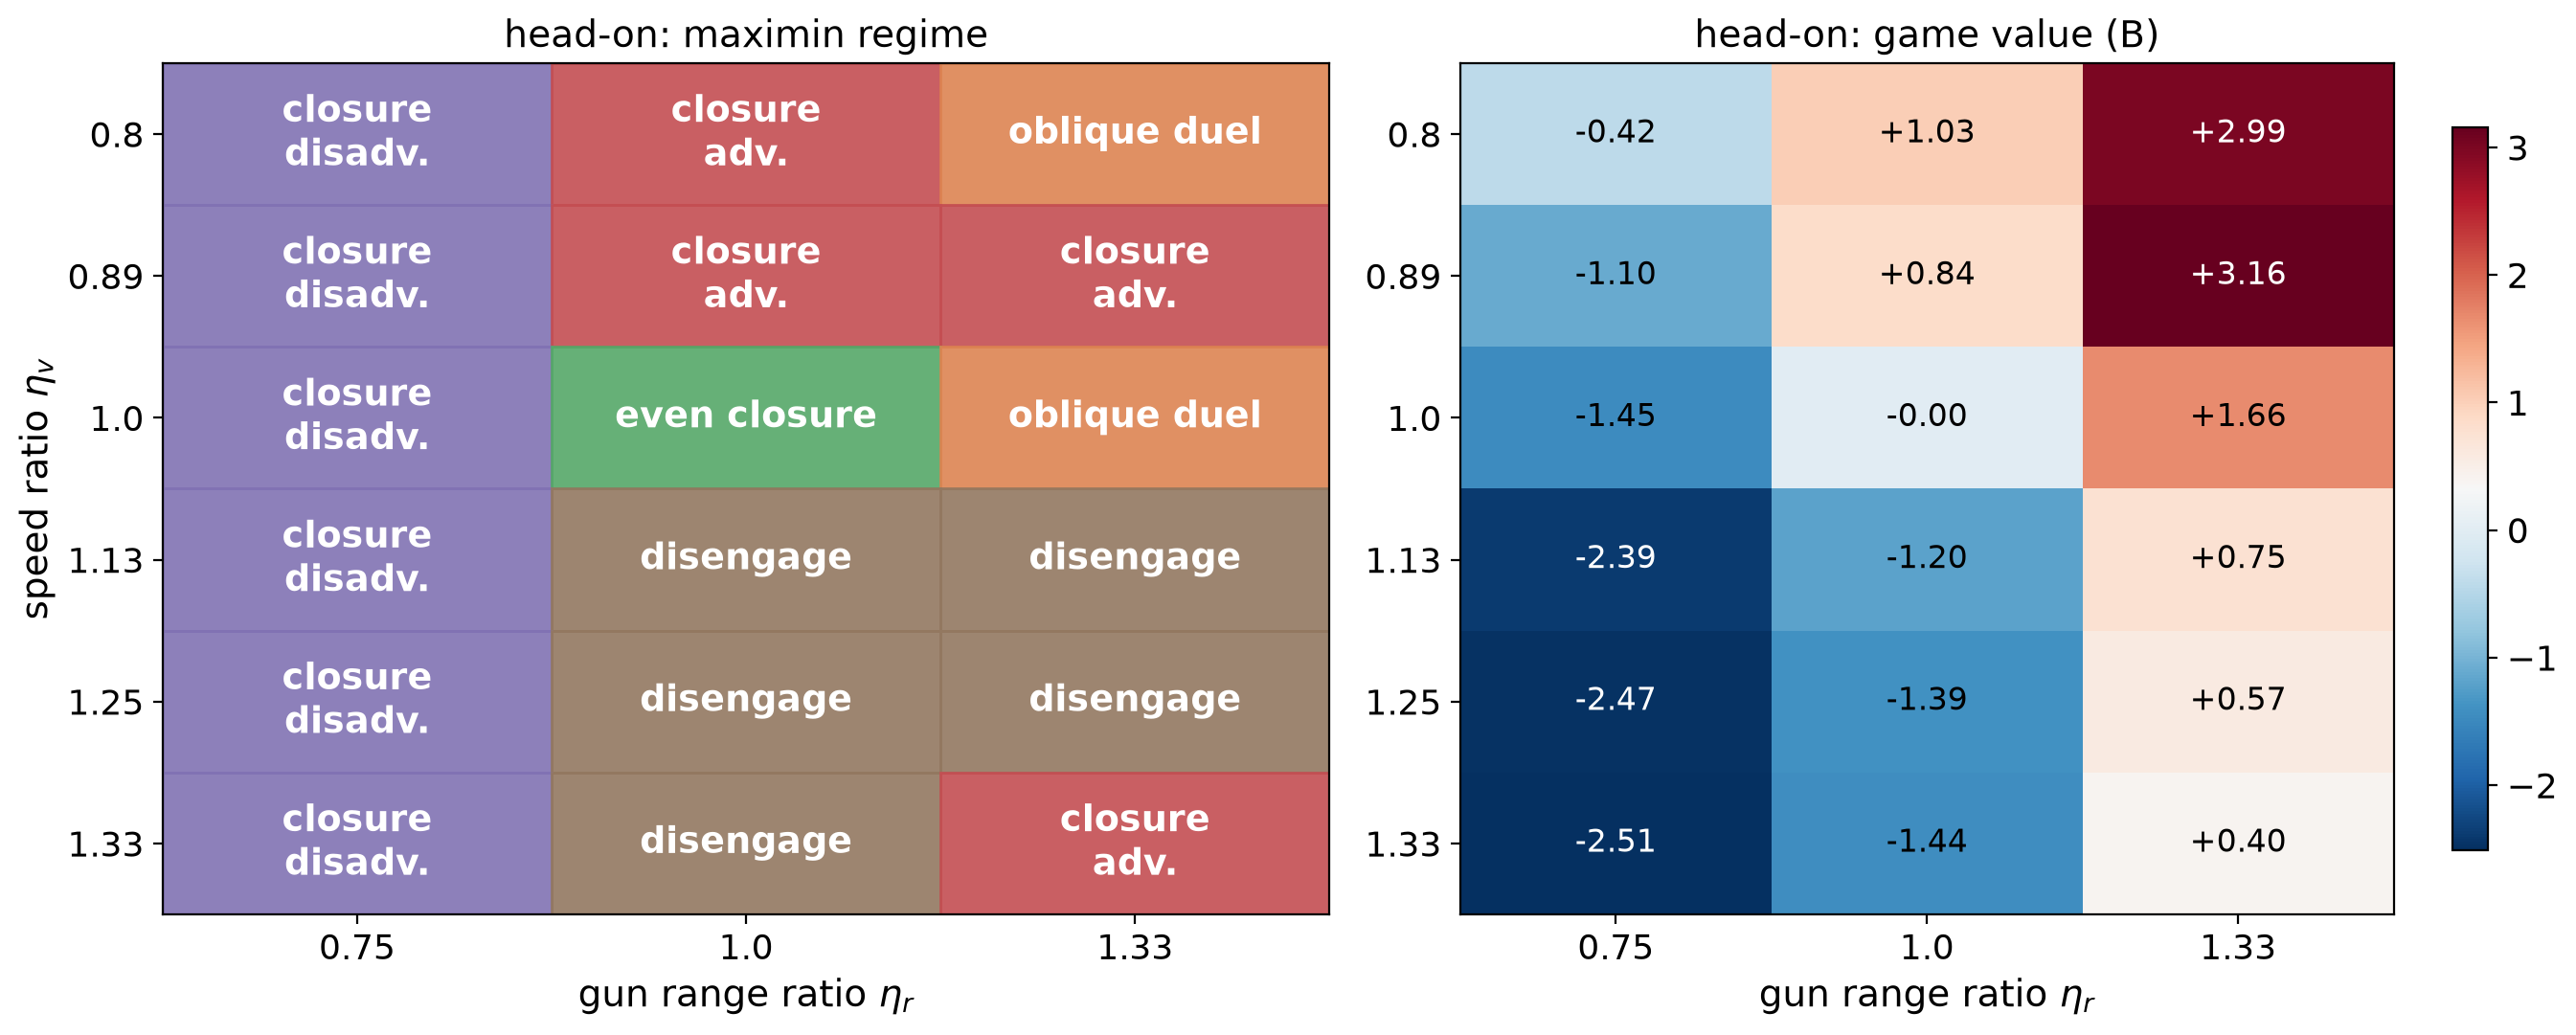
\includegraphics[width=0.98\textwidth]{figures/fig_e02_phase_head_on.png}\\
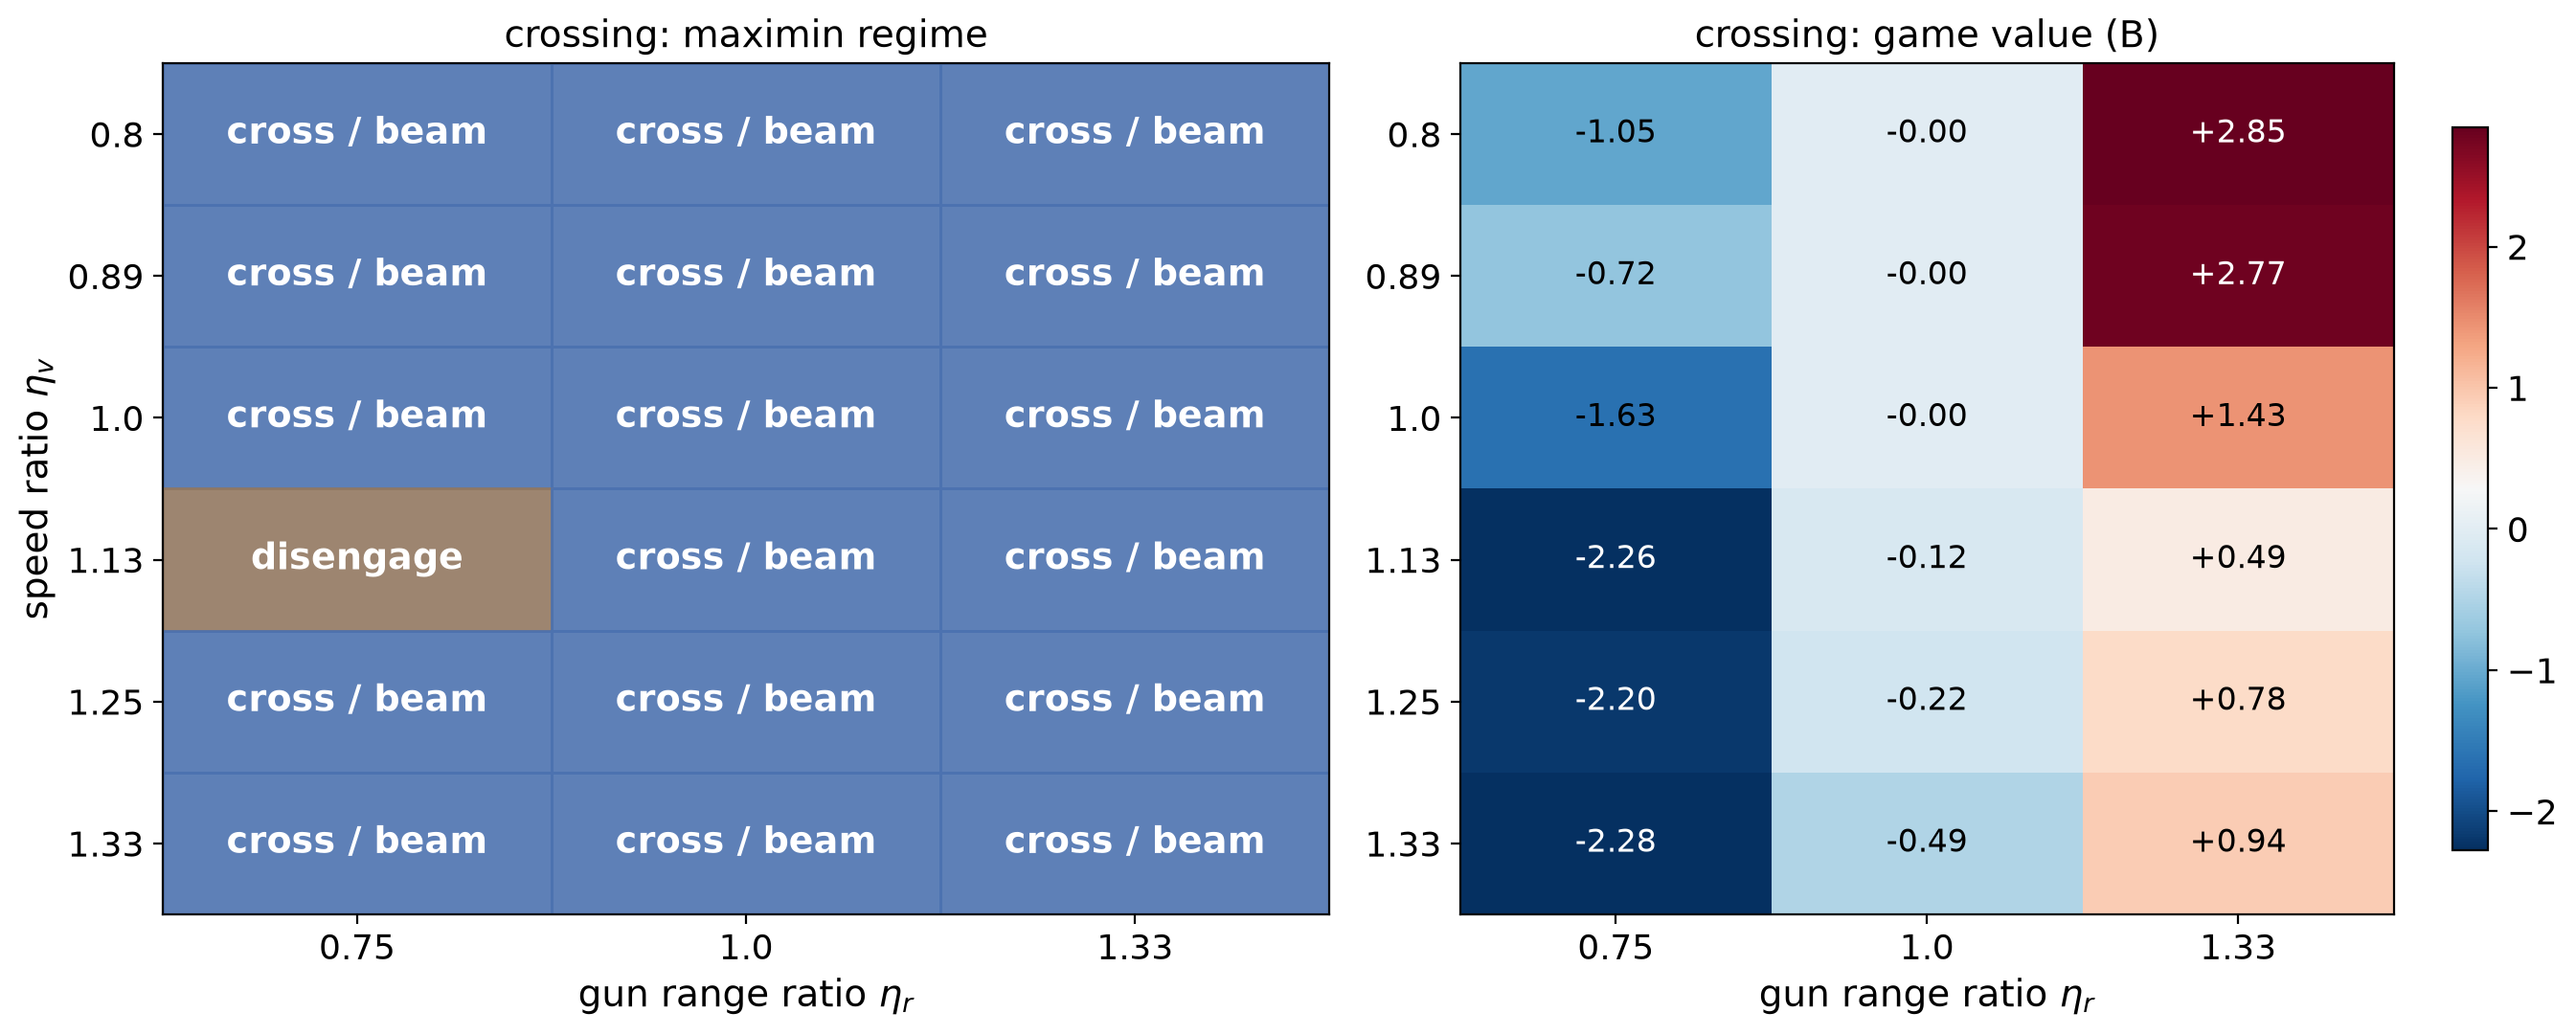
\includegraphics[width=0.98\textwidth]{figures/fig_e02_phase_crossing.png}
\caption{E02 三种初始几何下（速度比 $\etav$、炮程比 $\etar$）的战术区间
相图。每对的左图：maximin 承诺方案的主导区间；右图：B 的混合策略博弈值。}
\label{fig:phase}
\end{figure}

\begin{figure}[!htb]
\centering
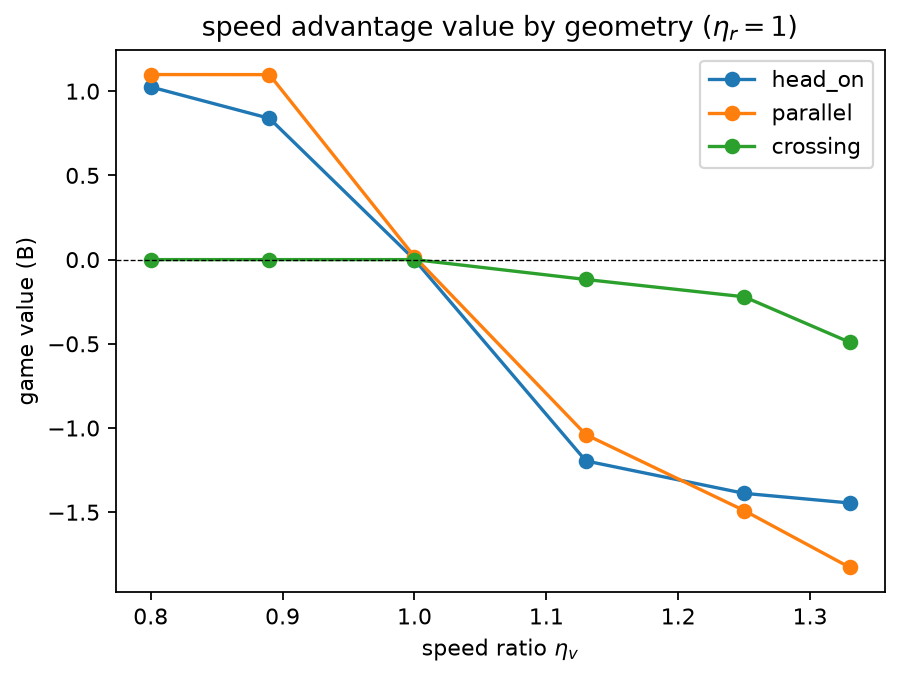
\includegraphics[width=0.6\textwidth]{figures/fig_e02_speed_mechanism.png}
\caption{速度机制分析（由 E02 脚本生成）：$\etar=1$ 时博弈值沿速度比轴的
变化。符号变化由 maximin 方案的离散区间切换产生，而非连续汇率平移。}
\label{fig:speed}
\end{figure}

\section{鱼雷机动剥夺（E04）}\label{sec:torpedo}

计划的核心假设（H2）为 $V_{\text{鱼雷}} = V_{\text{直接}} + V_{\text{剥夺}}$，
剥夺由目标的最优反应严格定义：$V_{\text{剥夺}} = J(\tau_0^*) - J(\tau_T^*)$，
其中 $J$ 是目标的炮位价值（假想终点上 \texttt{ship\_gun\_pressure}，即自身的
期望火力覆盖），$\tau_0^*,\tau_T^*$ 分别是无鱼雷与有鱼雷危险场时的最优机动
方案。关键在于：目标的决策目标只含概率性威胁——从不包含杀伤或教义项——因此
纯威胁区间（计划条件 D）按构造可用，分解不可能通过奖励设计伪造。

\paragraph{协议。} 一艘驱逐舰（吹雪级，九○式鱼雷）在四种初始几何（追击、
相向、斜交、近距）与两种兵力比（1v1、2v1）下攻击一艘重巡洋舰
（Northampton 级），每格 36 个配对种子（288 个测量样本）。双方先以固定直航
方案经引擎正式 submit/advance 管线航行一个回合（零掷骰：A/C/D 条件共享逐
字节相同的状态）；在鱼雷规划阶段枚举攻击者的全部合法发射空间（发射管 $\times$
舷侧 $\times$ 角度 $\times$ 速度档 $\times$ 发射脉冲，逐个经
\texttt{validate\_orders} 验证），每条航迹由引擎自身的脉冲环模型投影（与一次
真实裁决发射逐格核对），并在有无危险场的条件下在目标的完整合法方案空间
（340--600 条）上重算其最优反应。威胁权重 $w=0.343$ 是引擎碰撞表对目标排水量
档的期望毁伤比例（36 结果枚举）；$w=1$（计划的原始形式）作为敏感性报告。

\paragraph{结果。} 在\emph{低直接命中}子集
（$\mathbb{E}[\text{命中}] = 0.083$；$n=216$）中，$V_{\text{剥夺}}$ 结构性
恒等于零——全部 216 个样本恰为 $0$（bootstrap 区间退化为 $[0,0]$）——在
\emph{所有}几何与全部威胁权重下（$w=0.343$、$w=1$、常数威胁条件 D）皆然。
预置验收（至少三个几何的剥夺 CI 高于零）因此\textbf{失败}，我们连同机制如实
报告该零结果。机制是定量且具有一般性的：引擎命中表的粗粒度使目标的炮位价值
景观\emph{呈阶梯状}——每个测量的方案空间含 340--600 条合法方案，$J$ 在其中
平均只有 8 个不同取值（各格 4--14 个），且顶层（$J/J_{\text{ref}}=1$）平均被
25.5 条并列路线共享（各格 12--32.5）。单条鱼雷航迹是
$(\text{格},\text{脉冲})$ 空间中的一条细线：它能与顶层路线的\emph{部分}成员
相交，但永远无法覆盖整个顶层，于是目标免费重优化到一条并列路线（改航是真实
的——$100\%$ 样本改变航向、平均 $1.67\times60°$——但 $J$ 不变）。顶层下的
威胁折价期望成本（$w\cdot P_{\text{命中}} \approx 0.343\times0.083 \approx
0.029$）比阶梯落差（$0.58$）低一个数量级，故结论对威胁加权不变。

在\emph{直击}对照（$\mathbb{E}[\text{命中}]\in[0.42,1.14]$；$n=72$）中，
航迹直接压在顶层位置簇上，剥夺价值出现：$V_{\text{剥夺}} = 0.92$ 个价值点
（$95\%$ CI $[0.42, 1.42]$；归一化 $0.0264$），而改航反而变少（$15.3\%$）——
整个顶层簇被定价出局后，不存在并列避难所。分解
$V_{\text{鱼雷}} = V_{\text{直接}} + V_{\text{剥夺}}$ 本身得到确认：两个分量
均可测量、互不重叠，且低命中鱼雷的价值就是纯直接价值
（$V_{\text{鱼雷}} = 0.0285 = V_{\text{直接}} + 0$）。

\begin{figure}[!htb]
\centering
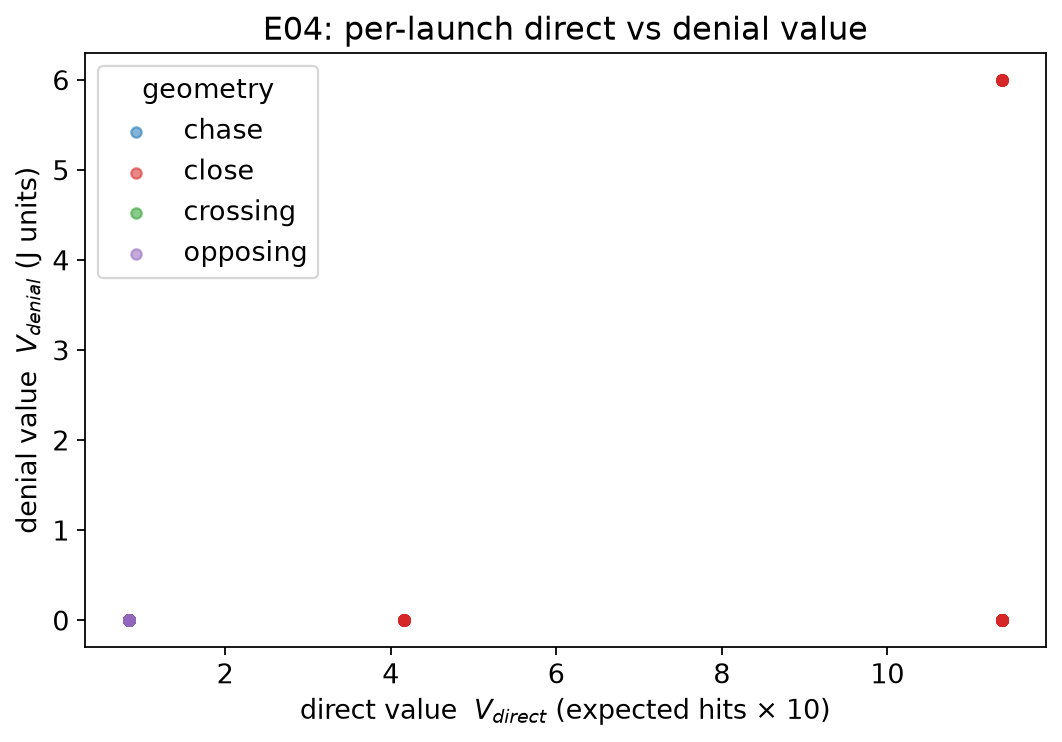
\includegraphics[width=0.62\textwidth]{figures/fig_e04_decomposition.png}
\caption{E04。逐次发射的直接价值对剥夺价值（直接价值以期望命中
$\times 10$ 为单位）：剥夺集中在直击（近距）几何，而低直接命中发射
（横轴近零）没有剥夺。}
\label{fig:e04}
\end{figure}

\paragraph{与预分析计划的偏离及设计混淆。} 测量前发生了两处协议偏离并记录在
仓库的实验日志中：(i)~原计划的``第 1 回合发射、第 2 回合响应''设计被证明
结构性不可行——约 700 个候选几何的 pilot 扫描显示第 1 回合航迹已经扫过目标
第 2 回合的可达集，所有接触都坍缩为近距舷侧直击——因此协议测量同回合完美
信息响应，与引擎自身的鱼雷辅助拦截模型同构；(ii)~几何由同一 pilot 扫描选定
以使稳定的低命中机会池存在。分析门限在本报告的测量之前已固定于项目的计划
文档与脚本中；未使用外部注册库。两项设计混淆限定直击对照：它来自单一几何
（近距），同时改变了距离、命中期望与航迹-阶梯重叠；且低命中池的
$\mathbb{E}[\text{命中}]$ 恒为 $1/12$（零方差），故``低命中区间''是命中分布
上的单点。区分这些因素的几何$\times$齐射规模因子实验是自然的延伸。

\paragraph{齐射规模扫描（E04c）。} 以威胁厚度为自变量直接识别机制。将攻击者
的发射按期望命中排序并组合前 $k$ 条航迹（$k=1,2,4,6$；每几何 30 个配对种子、
270 个去重测量、决策级协议）：直接价值随 $k$ 线性增长（均值 $2.6\to5.1\to
10.2\to20.2$ 个目标价值点），而剥夺单调但凸地上升
（$2.0\to2.0\to3.3\to5.0$），改航率只在 $k=6$ 达到 $100\%$。低命中层中剥夺
价值对厚度单调：$k\le2$ 时为 $0$（$n=60$）、$k=4$ 时 $+2.0$（$n=60$）、
$k=6$ 时 $+4.0$（$n=30$）。精化后的 H2 陈述——``薄的低命中威胁没有剥夺
价值；厚度才是购买它的货币''—— thus 直接可见于数据，附带精确阈值依赖于
威胁加权归一化的注意。

\begin{figure}[!htb]
\centering
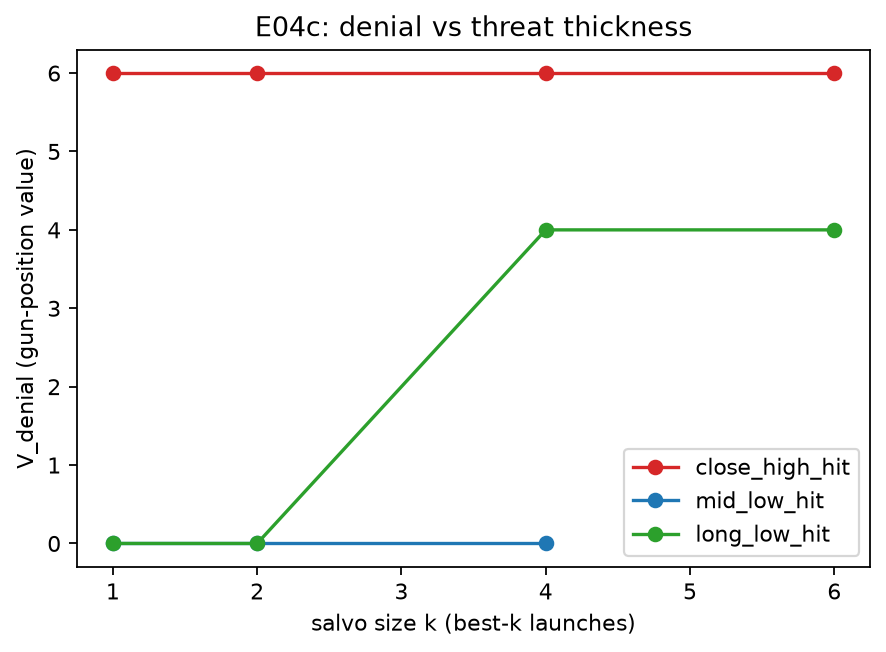
\includegraphics[width=0.6\textwidth]{figures/fig_e04salvo_curve.png}
\caption{E04c：各几何的剥夺价值对齐射规模 $k$。剥夺立即饱和而直接价值线性
增长；低命中层在 $k\le2$ 无剥夺、$k=4$ 为 $+2.0$、$k=6$ 为 $+4.0$。}
\label{fig:e04c}
\end{figure}

\paragraph{解读。} ``未命中但改变战局的鱼雷''在本引擎中确实发生——表现为
保持炮位价值的改航。薄的低概率威胁对阶梯化价值景观的剥夺价值恰为零；只有
当威胁覆盖目标的整个顶层位置簇（近距大规模齐射，或常数威胁感知区间 D——
同一批航迹在该区间给出 $V_{\text{剥夺}}^{(D)}=0.2126$）时剥夺价值才兑现。
这将 H2 精化为可检验的结构性主张：剥夺价值由威胁厚度与位置价值景观并列结构
的交互决定，而非命中概率单独决定。

\section{引擎在环验证（E06）}\label{sec:validation}

连续策略经\emph{几何策略}翻译为合法引擎命令：每个机动规划阶段它测量真实
几何，重解承诺机动博弈（滚动时域、三回合承诺），并在引擎自身的合法机动候选
中选取最匹配 maximin 航向变化且保持航速的方案；炮击目标最大化期望命中
$\times$ 目标价值。翻译由引擎的命令校验器审计；不改引擎状态、不读隐藏信息。

我们在近对称重巡决斗（San Francisco 级对 New Orleans 级）的三种初始几何下
验证，每格 60 个配对种子，ALLIES 一方始终是成熟的 \emph{balanced} 教义指挥
官；三个对比策略全部执 AXIS 一方（因此下文 ``vs.\ line'' 与 ``vs.\
straight'' 是替代 AXIS 策略，各自面对同一 \emph{balanced} 对手）。对不机动
的 \emph{straight} 基线，几何策略在每个几何都产生大而显著的配对战损差：
平行 $+7.7$ [$+6.4,+9.0$]（$93\%$ 配对为正）、斜交 $+9.6$ [$+8.1,+11.0$]
（$93\%$）、迎头 $+5.2$ [$+3.6,+6.8$]（$78\%$）。对教义档案的图景是差异化
且诚实的：九个配对格中唯一 $95\%$ 区间不含零的教义格是\emph{迎头 vs.
line}——纵队专家\emph{胜过}几何策略（$-1.73$ [$-3.23,-0.28$]；未校正，九
分之三之一）；其余各处策略与教义指挥官持平（其余 CI 全部含零；对
\emph{balanced} 的斜交格 $+1.47$ [$-0.03,+3.02$] 为边缘）。公平的总结是：
与成熟启发式持平——与简并命题的预测形状一致：对称决斗中成熟启发式已捕获
大部分位置价值，代理的贡献是从第一性原理\emph{保证}合格几何，而非 domination。
图~\ref{fig:e06} 给出配对森林图。

\paragraph{历史外部效度检查（E07）。} 作为合成几何之外的定性检查，同一翻译
层在历史埃斯佩兰斯角想定（IBS-S-01，历史特例规则生效：盟军火力减半、轴心
首回合禁射、盟军增援）中执日本一方，每策略 20 个种子。结果与合成验证一致并
更锐利：几何策略对 straight 基线的战损差为 $+12.2$ 个船体点（$95\%$ CI
$[+6.5,+17.9]$，$86\%$ 配对为正），对 \emph{line} 教义领先 $+3.7$
（$[-2.4,+9.6]$）——正趋势但未达显著。所有策略下轴心全负（胜率 $0\%$），
与引擎自带基准中该想定已知的盟军偏置一致（盟军 484 对轴心 174 个决定性胜局；
\texttt{benchmarks/ibs-s01-r30/README.md}），故胜负栏不用于任何战术结论。

\begin{figure}[!htb]
\centering
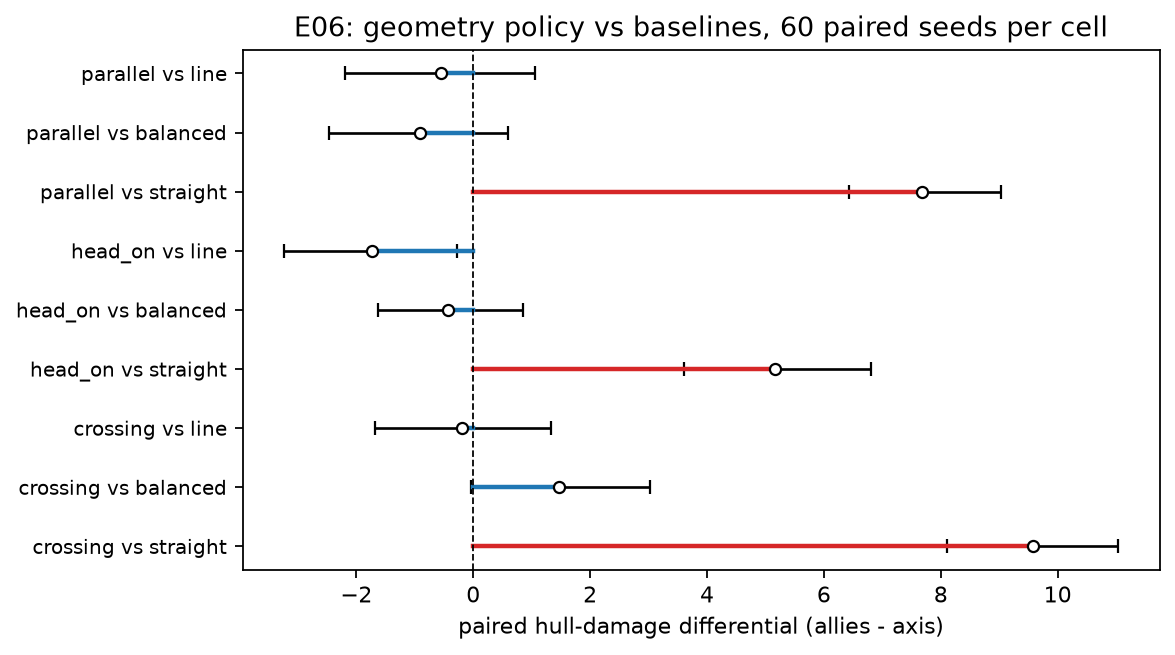
\includegraphics[width=0.8\textwidth]{figures/fig_e06_forest.png}
\caption{E06 配对验证。平均配对战损差（盟军减轴心；正值有利于几何策略）及
bootstrap $95\%$ CI，每格 60 个配对种子。}
\label{fig:e06}
\end{figure}

\section{几何诱导交战网络：一项规范分析（E05）}\label{sec:engagement}

计划假设（H3）：几何诱导的网络特征（局部兵力比、攻击者集中度、编队代数
连通度）对下一阶段战损的预测力超过总兵力/总火力，验收为 $\Delta R^2\ge
+0.05$ 或 MAE 改善 $\ge10\%$。我们运行 120 局（600 个回合快照；5{,}862 个
舰-回合样本；战损窗口与事件负载交叉核对，2{,}535/2{,}535 船体点），在夜战
可见性门控下以引擎真值期望火力边权构建有向图，并在 80/20 按局划分上比较 OLS
模型。

结果：加入图特征得到 $\Delta R^2=+0.0330$（$95\%$ CI $[+0.0069,+0.0561]$）
与 logistic 判别 AUC 增益 $+0.0286$（$[+0.0119,+0.0459]$），但 MAE 略
\emph{变差}（$-0.011$ $[-0.037,+0.015]$）。

然而，结论对规范选择敏感，且计划自身的指标列表解决了这一歧义：计划的
\S6.2 将图指标定义为包含\emph{加权入度}（$P_B(j)$，入射方向性期望火力）——
因此在计划字面读法下，基线只能包含非图总量（船体比例、航速、平均敌距、兵力
比），所有方向性火力量都属于图集合。以可复现脚本
\texttt{e05\_spec\_analysis.py}（比赛级 bootstrap，500 次重采样；点估计已
存档）在该计划字面规范下重新估计，交战图通过双重门限：$\Delta R^2 = +0.108$
（$95\%$ CI $[+0.069,+0.160]$），相对 MAE 降低 $17.5\%$（$95\%$ CI
$[9.7\%,26.7\%]$）。诚实的总结：\emph{方向性入度就是图}。一旦按计划指标列表
将其视为网络量，几何诱导交战网络在聚合兵力比之外具有可观的预测价值，而纯
\emph{形状}精化（局部兵力比、集中度、代数连通度）在其之外几乎没有增量；在
把入度计入基线的更严格读法下只剩形状特征，其增量 $+0.033$
（$[+0.007,+0.056]$）低于门限、MAE 略差。两种规范、点估计与两种 bootstrap
协议（样本级与比赛级）均在仓库中报告，读者可自行取舍。跨想定的样本外迁移
为负（S-01 训练测 S-03 及反向），把主张限定在同想定内预测。

\begin{figure}[!htb]
\centering
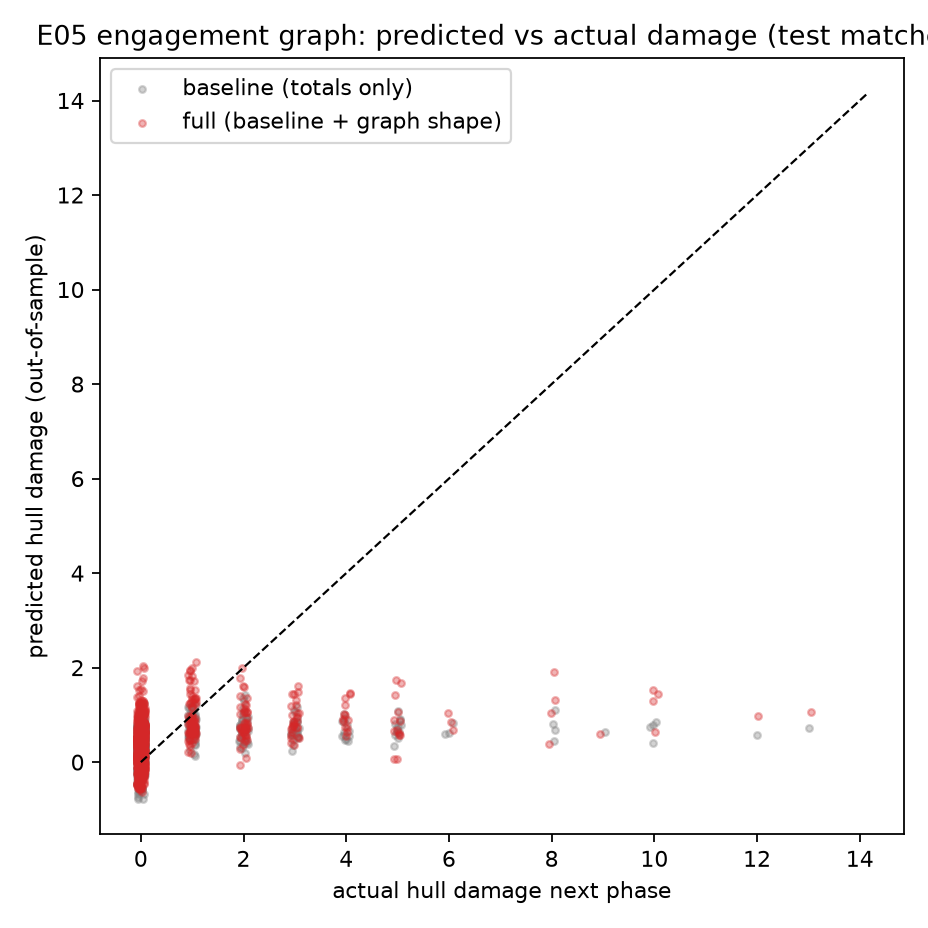
\includegraphics[width=0.49\textwidth]{figures/fig_e05_scatter.png}
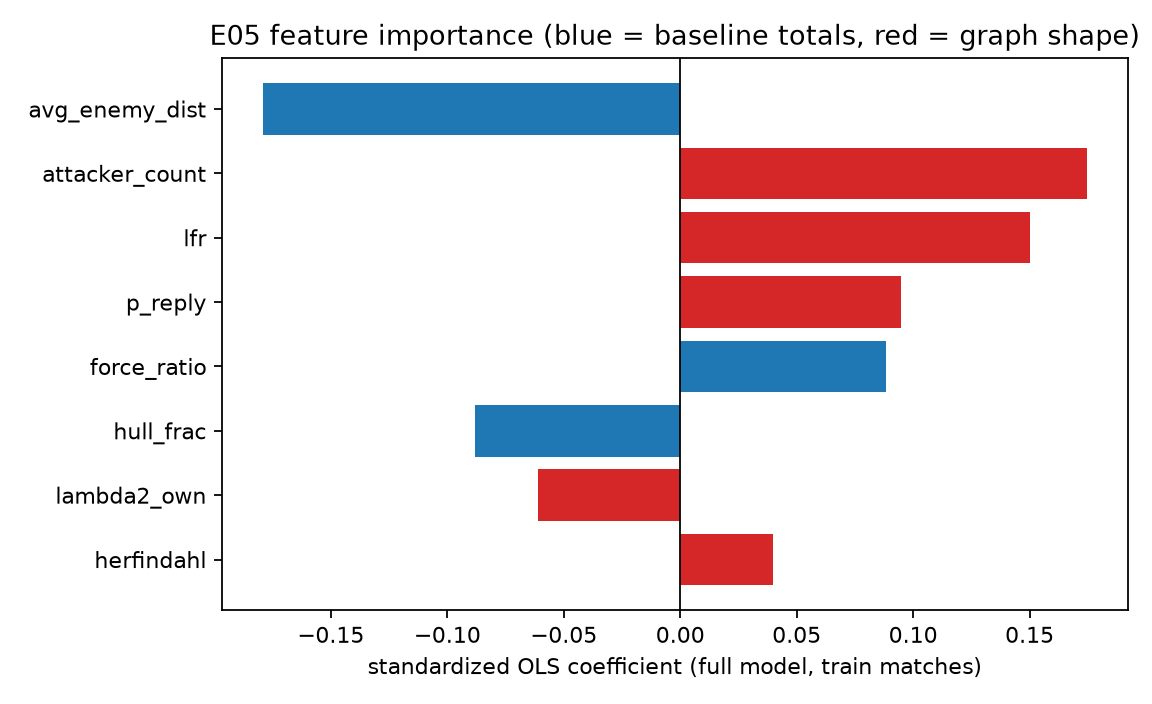
\includegraphics[width=0.49\textwidth]{figures/fig_e05_feature_importance.png}
\caption{E05。左：预测对实际下一阶段船体损伤（含图特征模型）。右：标准化 OLS
系数（蓝 = 基线总量，红 = 图形状特征）。}
\label{fig:e05}
\end{figure}

\section{讨论}\label{sec:discussion}

\paragraph{教义为何存在。} 简并命题给出对``为什么抢 T 是教义而非均衡策略''
的紧凑回答：闭环中，面对自由而知情的对手，位置机动一文不值；只有当方案被
承诺（如真实海战与引擎的密封命令）、能力不对称（速度、射程、火力）或信息
不完全时，它才变得有价值。开环分析随之定位了经典机动\emph{在哪里}最优
（图~\ref{fig:phase}）。

\paragraph{核买到了什么。} 一个 $\rho\approx0.99$ 保真度的光滑方向性代理使
微分博弈机制对完整离散规则集可用；反演 + 删失回归校准是通用的：任何表驱动
引擎都可以照此代理。

\paragraph{局限。} (i)~代理按舰种对在开阔水几何上校准；地形、烟雾、雷达
照明与编队效应不在 $L$ 中。E01b 的各向同性核对照与六项跨舰对迁移界定了
校准所证明的范围，但轴向行走方位基线与更多未见舰对仍是未来工作。
(ii)~方案库较粗；更细的自适应方案族会锐化区间边界。
(iii)~定速巡航近似忽略了航速节流战术（鱼雷的减速规避属 E04 管辖，由危险场
建模）。
(iv)~历史想定的特例规则部分执行（见引擎覆盖台账）；因此我们在合成对称交战
上验证，而非声称的历史复演。
(v)~相图中\emph{较慢}一方的微小正值（如 $\etav=0.8,\etar=1$ 时的 $+1.1$）
反直觉；它们源于承诺方案矩阵上的混合策略值在代理的穿越运动学（无碰撞、距离
下限半格）破坏交换对称时的产物——我们将其标注为待碰撞感知处理的模型伪影，
而非战术主张。
(vi)~引擎是兵棋而非物理：结论针对规则系统，历史教义只作定性外部锚。

\section{可复现性}\label{sec:repro}
每个实验都是 \texttt{research/experiments/} 下的脚本
（\texttt{e00\_engine\_audit}、\texttt{e01\_fire\_kernel}、
\texttt{e01b\_kernel\_baselines}、\texttt{e02\_crossing\_t\_phase}、
\texttt{e04\_torpedo\_denial}、\texttt{e04c\_salvo\_sweep}、
\texttt{e05\_engagement\_graph}、\texttt{e06\_engine\_validation}、
\texttt{e07\_historical\_check}），向 \texttt{research/results/} 写出原始
CSV/JSON 与图。全部运行带种子；配对比较共享想定、种子与初始布阵；置信区间
为 bootstrap 或精确（矩阵博弈 LP）。本文每个数字对应的冻结引擎提交为
\texttt{fc77a65}（\url{github.com/fuxiaoji/iron-bottom-sound}）。引擎提交、
规则覆盖台账与研究层纪律（不改裁决、不用隐藏信息、目标中无战术项）由 E00
审计。

\section{结论}
方向性火力、承诺机动与鱼雷威胁可以在一个完整确定性兵棋引擎作为校准与验证
基底时被当作同一个可测量系统来研究。校准核达到 $\rho=0.99$ 保真度；简并命题
解释了海军战术为何是承诺，以及对称决斗上的 RL 能学到什么、不能学到什么；
承诺机动博弈绘制了速度与射程不对称下的战术区间；翻译后的几何策略在引擎验证
中经受住教义基线的对抗；交战网络分析在其自身度量定义下通过门限，并给出其
规范边界；鱼雷剥夺零结果精确定位了教义直觉超出规则结构之处。我们把这条
管线——引擎、核、承诺机动博弈、翻译层、审计——视为持久贡献。

\appendix
\section{拟合距离修正量与引擎带的对照}
\label{app:modifiers}
表~\ref{tab:appendix-modifiers} 对每个攻击舰种比较核的拟合距离修正曲线
$M_r$（在引擎七个带中心取值）与引擎离散带值。远程带处 $\approx$+1.2 点的
残差偏移在四个舰种间共同（长程带为 5.17--5.24），与被吸收的常数修正一致而
非逐舰效应；拟合曲线的舰间一致性（如带 1：$-24.8$ 至 $-24.9$）是校准的
自检。

\begin{table}[h]
\centering\small
\caption{引擎带中心处拟合的 $M_r$（主炮、中性目标航速、舷侧姿态）对引擎
离散带值。}
\label{tab:appendix-modifiers}
\begin{tabular}{lccccccc}
\toprule
带中心（格） & 1 & 2 & 4 & 7.5 & 12.5 & 18 & 22+ \\
引擎带值 & $-24$ & $-15$ & $-12$ & $-6$ & $0$ & $+2$ & $+4$ \\
\midrule
DD（Laffey） & $-24.9$ & $-16.4$ & $-13.3$ & $-4.8$ & $+1.3$ & $+3.2$ & $+5.2$ \\
CL（Helena） & $-24.8$ & $-16.5$ & $-13.4$ & $-4.8$ & $+1.2$ & $+3.2$ & $+5.2$ \\
CA（San Francisco） & $-24.9$ & $-16.4$ & $-13.4$ & $-4.8$ & $+1.2$ & $+3.2$ & $+5.2$ \\
BB（Yamato） & $-24.8$ & $-16.5$ & $-13.4$ & $-4.8$ & $+1.2$ & $+3.2$ & $+5.2$ \\
\bottomrule
\end{tabular}
\end{table}

\section{逐舰种核图（DD、CL、BB）}
\label{app:polars}
图~\ref{fig:app-polars} 以剩余攻击舰种的校准核图补全图~\ref{fig:kernel}
（正文展示 CA）。舰种签名可见于各向异性：驱逐舰的火力集中于短程且呈近似
对称的四瓣结构，轻巡洋舰呈经典的全舷侧蝶形，战列舰远程更强且舰尾扇区缺口
显著。

\begin{figure}[h]
\centering
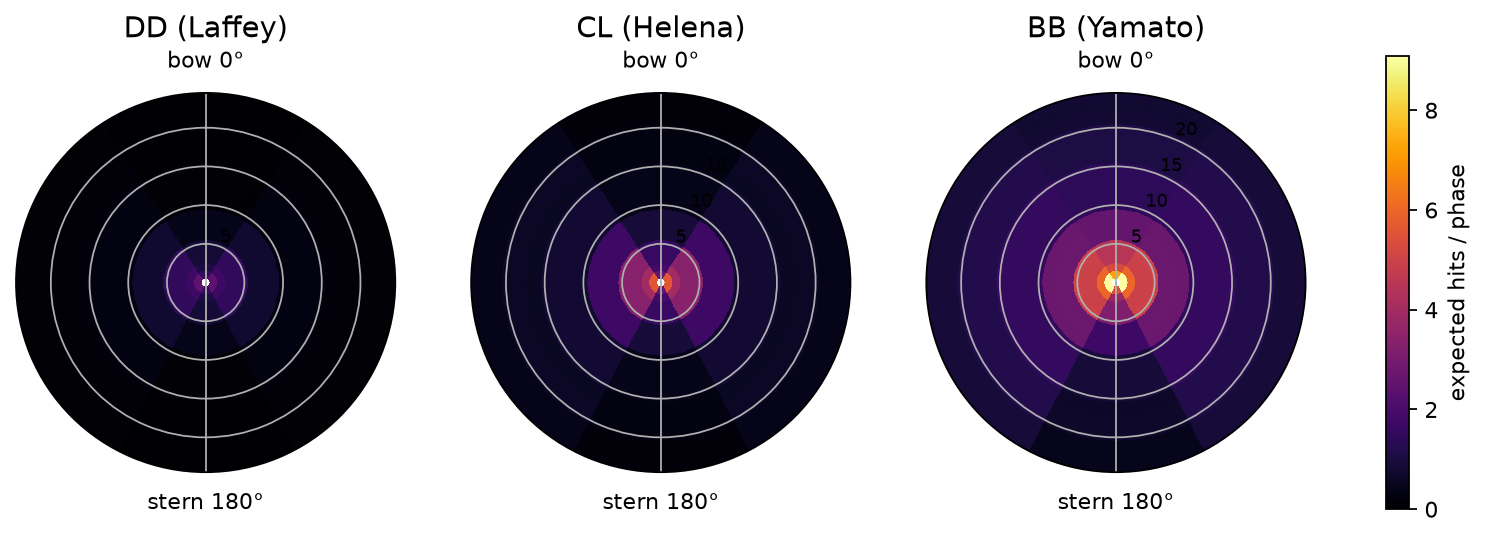
\includegraphics[width=0.85\textwidth]{figures/fig_e01_polars_appendix.png}
\caption{各舰种校准核图 $K(r,\theta)$（中性目标航速）。左：驱逐舰
（Laffey）。中：轻巡洋舰（Helena）。右：战列舰（Yamato）。}
\label{fig:app-polars}
\end{figure}

\begin{thebibliography}{20}

\bibitem{bernotti1911}
R.~Bernotti, ``The fundamentals of naval tactics,'' \emph{U.S. Naval
Institute Proceedings}, vol.~37, 1911.

\bibitem{bernotti1912}
R.~Bernotti, ``The fundamentals of naval tactics (continued),'' \emph{U.S.
Naval Institute Proceedings}, vol.~38, 1912.

\bibitem{taylor1974}
J.~G. Taylor, ``Lanchester-type models of warfare and optimal control,''
\emph{Naval Research Logistics Quarterly}, vol.~21, no.~1, pp.~79--106,
1974.

\bibitem{protopopescu1989}
V.~Protopopescu, R.~T. Santoro, and J.~Dockery, ``Combat modeling with
partial differential equations,'' \emph{European Journal of Operational
Research}, vol.~38, no.~2, pp.~178--183, 1989.

\bibitem{gonzalez2011}
E.~Gonz{\'a}lez and M.~Villena, ``Spatial Lanchester models,'' \emph{European
Journal of Operational Research}, vol.~210, no.~3, pp.~706--715, 2011.

\bibitem{networked2020}
A.~C. Kalloniatis, K.~Hoek, M.~Zuparic, and M.~Brede, ``Optimising
structure in a networked Lanchester model for fires and man{\oe}uvre in
warfare,'' \emph{Journal of the Operational Research Society}, vol.~72,
no.~8, pp.~1863--1878, 2021.

\bibitem{solis2020}
C.~U. Solis and J.~B. Clempner, ``Ship differential game approach for
multiple players: Stackelberg security games,'' \emph{Optimal Control
Applications and Methods}, vol.~41, no.~1, pp.~312--326, 2020.

\bibitem{weintraub2020}
I.~E. Weintraub, M.~Pachter, and E.~Garcia, ``An introduction to
pursuit--evasion differential games,'' in \emph{Proc. American Control
Conference (ACC)}, pp.~1049--1066, 2020.

\bibitem{cubic1993}
E.~A. Galperin, ``The cubic algorithm for global games with application to
pursuit-evasion games,'' \emph{Computers \& Mathematics with Applications},
vol.~26, no.~6, pp.~13--31, 1993.

\bibitem{bansal2021}
S.~Bansal and C.~J. Tomlin, ``DeepReach: A deep learning approach to
high-dimensional reachability,'' in \emph{Proc. IEEE ICRA}, pp.~1817--1824,
2021.

\bibitem{lanctot2017}
M.~Lanctot et~al., ``A unified game-theoretic approach to multiagent
reinforcement learning,'' in \emph{Advances in Neural Information
Processing Systems (NeurIPS)}, 2017.

\bibitem{bighashdel2024}
A.~Bighashdel, Y.~Wang, S.~McAleer, R.~Savani, and F.~A. Oliehoek,
``Policy space response oracles: A survey,'' in \emph{Proc. IJCAI},
pp.~7951--7961, 2024.

\bibitem{wellman2024}
M.~P. Wellman, K.~Tuyls, and A.~Greenwald, ``Empirical game-theoretic
analysis: A survey,'' \emph{arXiv:2403.04018}, 2024.

\bibitem{omidshafiei2019}
S.~Omidshafiei et~al., ``$\alpha$-Rank: Multi-agent evaluation by
evolution,'' \emph{Scientific Reports}, vol.~9, p.~9937, 2019.

\bibitem{adam2021}
L.~Adam, R.~Hor{\v{c}}{\'i}k, T.~Kasl, and T.~Kroupa, ``Double oracle
algorithm for computing equilibria in continuous games,'' in \emph{Proc.
AAAI}, vol.~35, no.~6, pp.~5070--5077, 2021.

\bibitem{wez2022}
W.~Wu, J.~Shi, Y.~Wu, Y.~Wang, and Y.~Lyu, ``A multi-UCAV cooperative
occupation method based on weapon engagement zones for beyond-visual-range
air combat,'' \emph{Defence Technology}, vol.~18, no.~6, pp.~1006--1022,
2022.

\end{thebibliography}

\end{document}
